\documentclass[tikz,border=2mm]{standalone}
\usetikzlibrary{arrows.meta,calc}

\definecolor{manifoldFill}{RGB}{229,241,255}
\definecolor{manifoldDraw}{RGB}{57,98,150}
\definecolor{groupFill}{RGB}{236,248,236}
\definecolor{groupDraw}{RGB}{58,122,69}
\definecolor{flowRed}{RGB}{190,55,48}
\definecolor{actionPurple}{RGB}{105,77,168}
\definecolor{textGray}{RGB}{70,70,70}

\begin{document}
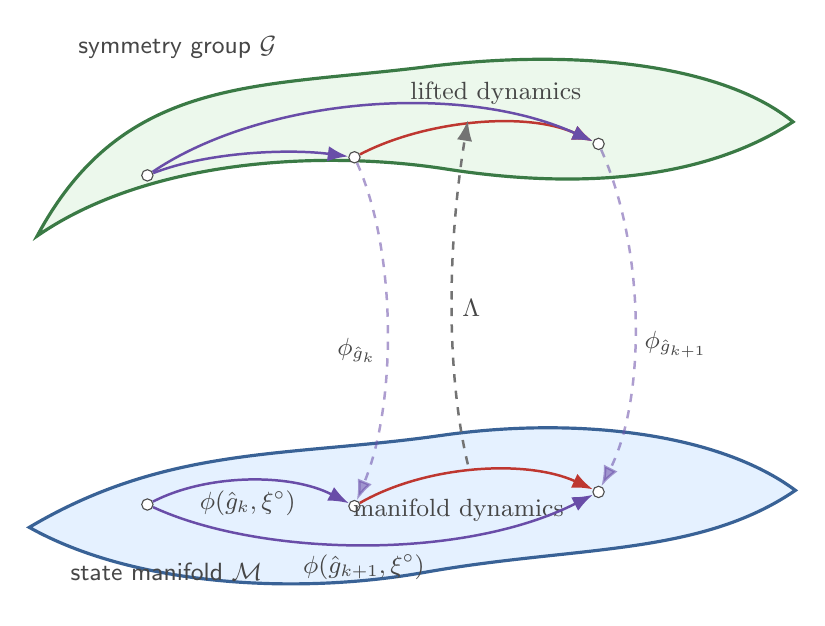
\begin{tikzpicture}[
  >=Latex,
  font=\sffamily,
  label/.style={font=\small\sffamily, text=textGray},
  mathlabel/.style={font=\small, text=textGray},
  state/.style={circle, draw=black!70, fill=white, inner sep=1.45pt},
  arrow/.style={line width=0.9pt, -{Latex[length=2.6mm]}},
  dyn/.style={arrow, draw=flowRed},
  action/.style={arrow, draw=actionPurple},
  lift/.style={arrow, draw=black!55, dashed}
]

% Hovering symmetry group.
\path[fill=groupFill, draw=groupDraw, line width=1.15pt]
  (-4.75,1.95)
  .. controls (-3.35,2.92) and (-1.15,3.05) .. (0.45,2.80)
  .. controls (2.25,2.52) and (3.78,2.70) .. (4.85,3.40)
  .. controls (4.00,4.10) and (2.20,4.35) .. (0.20,4.10)
  .. controls (-1.95,3.83) and (-3.65,4.00) .. (-4.75,1.95)
  -- cycle;
\node[label, anchor=west] at (-4.35,4.34) {symmetry group $\mathcal{G}$};

% Physical state manifold.
\path[fill=manifoldFill, draw=manifoldDraw, line width=1.15pt]
  (-4.85,-1.75)
  .. controls (-3.55,-2.48) and (-1.50,-2.62) .. (0.18,-2.32)
  .. controls (2.10,-1.98) and (3.65,-2.12) .. (4.88,-1.28)
  .. controls (3.90,-0.55) and (2.10,-0.34) .. (0.40,-0.58)
  .. controls (-1.55,-0.86) and (-3.08,-0.70) .. (-4.85,-1.75)
  -- cycle;
\node[label, anchor=west] at (-4.45,-2.32) {state manifold $\mathcal{M}$};

% Reference elements.
\node[state, label={[mathlabel]left:$\xi^\circ$}] (xref) at (-3.35,-1.46) {};
\node[state, label={[mathlabel]left:$I$}] (gid) at (-3.35,2.72) {};

% Estimates on group and manifold at two time steps.
\node[state, label={[mathlabel]above:$\hat{g}_k$}] (gk) at (-0.72,2.95) {};
\node[state, label={[mathlabel]above:$\hat{g}_{k+1}$}] (gkp1) at (2.38,3.12) {};

\node[state, label={[mathlabel]below:$\hat{\xi}_k$}] (xk) at (-0.72,-1.48) {};
\node[state, label={[mathlabel]below:$\hat{\xi}_{k+1}$}] (xkp1) at (2.38,-1.30) {};

% Dynamics arrows: same time step progression on both spaces.
\draw[dyn] (gk)
  .. controls (0.18,3.42) and (1.46,3.54) .. (gkp1)
  node[pos=0.58, above=3pt, mathlabel] {lifted dynamics};
\draw[dyn] (xk)
  .. controls (0.18,-0.96) and (1.46,-0.88) .. (xkp1)
  node[pos=0.43, below=6pt, mathlabel] {manifold dynamics};

% Group-action arrows from identity/reference to the corresponding estimates.
\draw[action] (gid)
  .. controls (-2.58,3.02) and (-1.55,3.06) .. (gk);
\draw[action] (xref)
  .. controls (-2.62,-1.08) and (-1.56,-1.05) .. (xk)
  node[midway, below, mathlabel] {$\phi(\hat{g}_k,\xi^\circ)$};

\draw[action] (gid)
  .. controls (-1.90,3.70) and (0.62,3.92) .. (gkp1);
\draw[action] (xref)
  .. controls (-1.92,-2.12) and (0.64,-2.18) .. (xkp1)
  node[midway, below, mathlabel] {$\phi(\hat{g}_{k+1},\xi^\circ)$};

% Vertical correspondences from group estimates to manifold estimates.
\draw[action, dashed, opacity=0.55] (gk)
  .. controls (-0.18,1.75) and (-0.18,-0.18) .. (xk)
  node[pos=0.56, left, mathlabel, opacity=1] {$\phi_{\hat{g}_k}$};
\draw[action, dashed, opacity=0.55] (gkp1)
  .. controls (2.98,1.78) and (2.98,-0.12) .. (xkp1)
  node[pos=0.56, right, mathlabel, opacity=1] {$\phi_{\hat{g}_{k+1}}$};

% Lift relation between the two dynamics arrows.
\draw[lift] (0.72,-0.95)
  .. controls (0.45,0.18) and (0.45,1.76) .. (0.72,3.42)
  node[midway, right, mathlabel] {$\Lambda$};

\end{tikzpicture}
\end{document}
